\section{PHACTS}

PHACTS\cite{mcnair2012phacts} là một trong những công cụ tiên phong trong việc phân loại thực khuẩn thể theo vòng đời dựa trên bộ gen đầy đủ. Công cụ này sử dụng thuật toán rừng ngẫu nhiên để xây dựng mô hình học máy dựa trên mức độ tương đồng protein giữa các thực khuẩn.

\subsection{Dữ liệu huấn luyện}
Dữ liệu huấn luyện được sử dụng trong bài báo là dữ liệu thu thập từ cơ sở dữ liệu PHANTOME, gồm 654 bộ gen thực khuẩn. Trong đó, dữ liệu được sử dụng cho huấn luyện gồm 227 thực khuẩn có vòng đời đã được xác nhận bằng phương pháp thủ công từ nhiều nguồn tài liệu khác nhau, cụ thể tập huấn luyện chứa 148 thực khuẩn thể ôn hoà và 79 thực khuẩn thể độc lực. Đặc điểm của tập dữ liệu này là tỷ lệ lớp không cân bằng (2:1), phản ánh đúng về sự phân bố dữ liệu của thực khuẩn thể ôn hoà trong dữ liệu.

Để đảm bảo tính khách quan trong đánh giá mô hình, các thực khuẩn có độ tương đồng cao về protein (>90\% protein giống nhau với >90\% độ tương đồng) với thực khuẩn đang được kiểm tra sẽ bị loại khỏi tập huấn luyện. Điều này giúp tránh tình trạng mô hình "học tủ" và đánh giá chính xác khả năng tổng quát hóa.

\subsection{Phương pháp}

\textbf{Tạo tập protein chuẩn} (\textit{query proteins}): Một tập hợp các chuỗi protein truy vấn \( Q = \{P_1, P_2, \ldots, P_M\} \) được tạo ra bằng cách chọn ngẫu nhiên \( M \) protein, trong đó \( M \) là số lượng protein do người dùng chỉ định để sử dụng cho việc tạo tập huấn luyện. Từ mỗi lớp, \( M/C \) protein được chọn ngẫu nhiên, thuộc về các thể thực khuẩn của lớp đó, với \( C \) là số lượng lớp trong tập huấn luyện. Trong các thí nghiệm của nhóm tác giả, việc chọn \( M = 600 \) cho kết quả tốt nhất được lựa chọn theo kinh nghiệm. Khi giảm giá trị \( M \), độ chính xác giảm xuống; ngược lại, khi tăng giá trị \( M \), thời gian chạy tăng lên mà không mang lại sự cải thiện tương ứng về độ chính xác.

\textbf{Tạo tập dữ liệu huấn luyện}: Để tạo tập dữ liệu huấn luyện cho thuật toán rừng ngẫu nhiên, một tập hợp gồm \( N \) vectơ tương đồng được xây dựng, trong đó \( N \) là số lượng thể thực khuẩn được sử dụng làm các trường hợp huấn luyện. Từ mỗi lớp, \( N/C \) bộ gen của thực khuẩn được chọn ngẫu nhiên mà không hoàn lại, với \( C \) là số lượng lớp. Từ \( N \) thực khuẩn này, danh sách \( L = \{G_1, G_2, \ldots, G_N\} \) được tạo ra. Lớp có số lượng mẫu đại diện ít nhất sẽ giới hạn số lượng trường hợp huấn luyện có thể sử dụng. Từ kinh nghiệm thực nghiệm của nhóm tác giả, giá trị \( N = 100 \) cho kết quả tốt nhất. Và với 50 thực khuẩn mỗi lớp là đủ để thu được kết quả chính xác đồng thời đảm bảo tính đa dạng trong việc lấy mẫu ngẫu nhiên. 

Đối với mỗi bộ gen trong số \( N \) bộ gen này, một vector tương đồng \( \mathbf{X} \) được xây dựng. Các protein của một thực khuẩn được so sánh với tất cả các protein trong tập \( Q \) bằng chương trình FASTA. Từ đó, vector tương đồng $X = [S_1, S_2, \dots, S_M]$ được xây dựng, trong đó $S_i$ là phần trăm độ tương đồng cao nhất giữa bất kỳ protein nào của phage đầu vào và protein chuẩn $P_i$ trong tập $Q$, như mô tả bên dưới:

\[
\mathbf{X}_1 = [S_{1,1}, S_{1,2}, \ldots, S_{1,M}]
\]
\[
\mathbf{X}_2 = [S_{2,1}, S_{2,2}, \ldots, S_{2,M}]
\]
\[
\vdots
\]
\[
\mathbf{X}_N = [S_{N,1}, S_{N,2}, \ldots, S_{N,M}]
\]

\textbf{Huấn luyện thuật toán rừng ngẫu nhiên}: Để phân loại tập kiểm tra, PHACTS sử dụng thuật toán rừng ngẫu nhiên. Trong bộ phân loại rừng ngẫu nhiên, một tập hợp các cây quyết định được tạo ra. Đối với mỗi cây, kỹ thuật bootstrapping được áp dụng bằng cách chọn \( N \) mẫu có hoàn lại từ tập huấn luyện gồm \( N \) mẫu. Mỗi cây được phát triển bằng cách chọn ngẫu nhiên \( m \) biến tại mỗi nút, trong đó \( m \) bằng căn bậc hai của tổng số biến. Phép tách tốt nhất tại nút đó được xác định từ tập \( m \) biến này, và cây được phát triển tối đa mà không bị cắt tỉa.

Mỗi cây đưa ra một dự đoán về chu trình (độc lực hay ôn hòa), và dự đoán cuối cùng được xác định bằng quy tắc bỏ phiếu đa số từ tất cả các cây trong rừng. Rừng ngẫu nhiên cũng cung cấp thông tin về tỷ lệ bỏ phiếu, được tính bằng phần trăm số lượng cây dự đoán một chu trình cụ thể chia cho tổng số cây. Vì thuật toán rừng ngẫu nhiên không dẫn đến hiện tượng quá khớp, nên có thể tạo ra số lượng lớn cây. Trong các thí nghiệm của nhóm tác giả, 1001 cây được tạo ra để đảm bảo đủ mức bao phủ cho tập huấn luyện.

\textbf{Cách đưa ra dự đoán chinh xác, ổn định}: Dự đoán thu được từ thuật toán rừng ngẫu nhiên với \( N \) thực khuẩn đã biết, được chọn ngẫu nhiên làm các trường hợp huấn luyện, và \( M \) protein, được chọn ngẫu nhiên để tạo các vector tương đồng. Do việc lựa chọn dữ liệu huấn luyện là ngẫu nhiên, một thực khuẩn chưa biết có thể bị dự đoán là thuộc các chu trình sống khác nhau trong các lần phân loại rừng ngãu nhiên khác nhau.

Để xử lý tốt hơn sự biến thiên này trong các dự đoán, nhóm tác giả thực hiện 10 lần lặp với các tập hợp thực khuẩn huấn luyện khác nhau và tập hợp protein truy vấn khác nhau. Mười lần lặp được chọn nhằm cân bằng giữa thời gian thực thi và độ chính xác. Các dự đoán dựa trên 5 lần lặp cho độ chính xác thấp hơn, trong khi dự đoán với 20 lần lặp làm tăng đáng kể thời gian thực thi mà không mang lại sự cải thiện tương ứng về độ chính xác.

Điểm xác suất cuối cùng được xem là “đáng tin cậy” nếu có sự đồng thuận từ 10 lần lặp cho một chu trình sống cụ thể. Để xác định liệu một dự đoán có đáng tin cậy hay không, giá trị trung bình và độ lệch chuẩn của 10 lần lặp được tính toán. Dự đoán được xem là đáng tin cậy nếu điểm xác suất trung bình của chu trình sống được dự đoán cao hơn 2 độ lệch chuẩn so với điểm xác suất trung bình của chu trình còn lại.

\textbf{Lọc đặc trưng quan trọng}: Để tăng độ chính xác và hiệu quả tính toán, PHACTS sử dụng phương pháp Gini Importance để đánh giá mức độ quan trọng của từng protein trong việc phân loại. Gini Importance đo lường mức độ đóng góp của một protein vào khả năng phân biệt giữa các lớp (ôn hòa và độc lực). Giá trị Gini Importance cao cho thấy protein đó có vai trò quan trọng trong việc phân loại và giá trị Gini Importance thấp cho thấy protein đó ít đóng góp vào việc phân loại. Chỉ các protein có Gini Importance vượt qua một ngưỡng nhất định (trong nghiên cứu là gấp đôi giá trị trung bình) mới được giữ lại để xây dựng vector tương đồng. Việc loại bỏ các protein ít quan trọng giúp giảm nhiễu, tăng tốc độ xử lý và cải thiện độ chính xác của mô hình.

\subsection{Kết quả và đánh giá}
Kết quả thực nghiệm của PHACTS:
    \begin{itemize}
        \item PHACTS đạt độ chính xác cao trong việc phân loại thực khuẩn.
        \item Độ chính xác: đạt 99\% (197/199 phage được phân loại chắc chắn). 
        \item Độ nhạy: đạt 88\%. 
        \item Đối với bộ gen không đầy đủ (chỉ sử dụng một phần protein), PHACTS vẫn duy trì được độ chính xác tương đối cao: xấp xỉ 90\% khi sử dụng khoảng 20 proteins.
    \end{itemize}

Từ các kết quả thực nghiệm cho thấy rằng, ưu điểm của PHACTS là có thể đưa ra dự đoán với độ chính xác chấp nhận được ngay cả khi chỉ có một phần bộ gen của thực khuẩn. Việc sử dụng mô hình Rừng ngẫu nhiên cũng giúp cho PHACTS dễ hiểu và có thể được giải thích một cách rõ ràng. Bên cạnh những ưu điểm, PHACTS cũng tồn tại hạn chế đáng kể. Mô hình học máy của PHACTS được huấn luyện trên một số lượng nhất định các thực khuẩn đã biết. Nếu gặp các thực khuẩn rất khác biệt, khả năng phân loại chính xác của PHACTS sẽ giảm.

\section{PhageAI}
PhageAI\cite{tynecki2020phageai} sử dụng phương pháp tiếp cận dựa trên học máy và xử lý ngôn ngữ tự nhiên để phân loại thực khuẩn dựa trên trình tự nucleotide. Quy trình giải pháp của PhageAI được mô tả trong Hình \ref{fig:phageai}
\begin{figure}[ht]
    \centering
    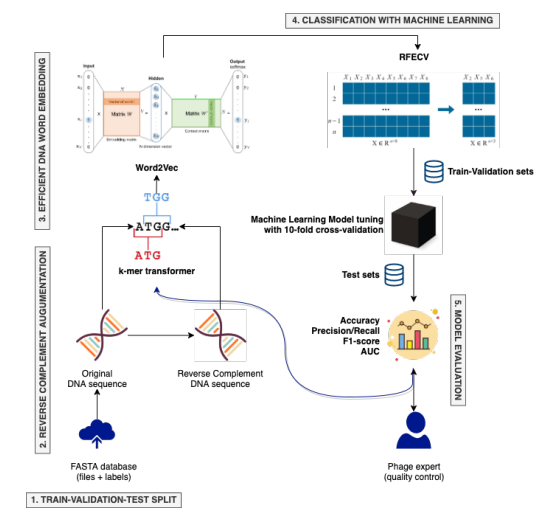
\includegraphics[width=0.8\linewidth]{figures/phageai.png}
    \caption{Quy trình giải pháp đề xuất của PhageAI}
    \label{fig:phageai}
\end{figure}

\subsection{Dữ liệu huấn luyện}
Trong nghiên cứu này, dữ liệu được thu thập từ hai cơ sở dữ liệu chuyên biệt về thực khuẩn thể là ACLAME và PhagesDB. Tổng cộng có hơn 600 bộ gen thực khuẩn. Trong đó mỗi mẫu đều được gán nhãn về chu kỳ sống — bao gồm chu kỳ tan tương ứng với thực khuẩn thể độc lực và chu kỳ tiềm tan tương ứng với thực khuẩn thể ôn hoà.

Tập dữ liệu được phân chia thành hai phần chính:(1) Tập huấn luyện Gồm 278 mẫu thực khuẩn thể độc lực và 174 mẫu thực khuẩn thể ôn hoà. (2) Tập kiểm tra gồm 54 mẫu thực khuẩn thể độc lực và 30 mẫu thực khuẩn thể ôn hoà, được lựa chọn từ các họ và loài thực khuẩn thể khác với các mẫu trong tập huấn luyện, nhằm đảm bảo khả năng tổng quát hóa của mô hình.


\subsection{Phương pháp}
\textbf{Phân chia dữ liệu huấn luyện}: Để kiểm soát và theo dõi quá trình học của mô hình phân loại, PhageAI sử dụng chiến lược phân chia dữ liệu như sau:
\begin{itemize}
    \item Tập huấn luyện: Dữ liệu được chia ngẫu nhiên thành 10 phần bằng nhau. Trong mỗi vòng lặp, 80\% dữ liệu được sử dụng để huấn luyện, và 20\% còn lại dùng để kiểm tra trong quá trình học. Việc phân tầng được thực hiện dựa trên vòng đời và họ của thực khuẩn, nhằm đảm bảo tính đại diện của các nhóm trong từng phần dữ liệu.
    
    \item Tập thử nghiệm: Một tập gồm 84 mẫu chưa từng được sử dụng trong quá trình huấn luyện được giữ lại để làm dữ liệu kiểm tra độc lập. Tập này được dùng để đánh giá khách quan hiệu suất của mô hình sau khi quá trình học kết thúc.
    
    \item Bộ dữ liệu kiểm tra bên ngoài: Một tập dữ liệu thứ hai gồm 61 mẫu, do công ty Proteon Pharmaceuticals S.A. cung cấp, cũng không được sử dụng trong giai đoạn huấn luyện. Tập này được dùng để ước lượng các chỉ số hiệu suất cuối cùng của mô hình khi áp dụng lên dữ liệu thực tế hoàn toàn mới.
\end{itemize}

\textbf{Tăng cường dữ liệu bằng phương pháp bổ sung chuỗi đảo ngược}: Sau khi phân chia dữ liệu, PhageAI áp dụng kỹ thuật tăng cường dữ liệu bằng cách sử dụng chuỗi bổ sung đảo ngược của các trình tự thực khuẩn như các mẫu bổ sung. Điều này cho phép mô hình học máy tự động học các mối quan hệ phức tạp giữa các trình tự DNA sợi đôi. Kỹ thuật này còn giúp tăng gấp đôi kích thước tập dữ liệu, từ đó cải thiện hiệu suất của mô hình.

\textbf{Phương pháp vector hóa}: Trình tự gen của thực khuẩn ở tệp tin dạng FASTA thường là các chuỗi tương đối dài (từ 5.000 đến 300.000 bp) bao gồm các nucleotide \{A, C, G, T\}. PhageAI đã áp dụng các kỹ thuật xử lý ngôn ngữ tự nhiên phổ biến để xây dựng không gian vector đại diện cho các trình tự thực khuẩn và giảm đáng kể yêu cầu bộ nhớ nhằm tăng tốc quá trình phân loại. Cụ thể, nhóm nghiên cứu đã sử dụng phương pháp biểu diễn phân tán của các thành phần k-mer chồng lấn và nhúng từ.

Để có được các vector đặc trưng có kích thước cố định đại diện cho các gen, nhóm nghiên cứu đã áp dụng phương pháp nhúng từ dựa trên Word2Vec với mô hình Skip-gram. Cuối cùng, DNA của thực khuẩn được biểu diễn bằng trung bình của các vector nhúng k-mer của các từ cấu thành trình tự, có nghĩa là mỗi gen được mô tả bằng các giá trị số trung bình trong không gian vector.

\textbf{Phân loại với Học máy}: Trong nghiên cứu này, các đặc trưng không đồng nhất được trích xuất từ trung bình của các vector nhúng k-mer có thể phản ánh thông tin mẫu tốt hơn. Vì mục đích này, nhóm nghiên cứu đã áp dụng RFECV (Recursive feature elimination with cross-validation), một phương pháp lựa chọn tính năng hiệu quả để loại bỏ các thuộc tính không liên quan và tăng khả năng tổng quát hóa của mô hình ở bước tiếp theo. Thông qua quá trình này, 150 đặc trưng quan trọng đã được chọn từ tổng số 300 đặc trưng để sử dụng trong quá trình phân loại.
Trong phạm vi bài báoo này, nhóm tả giả đã thực hiện huấn luyện và so sánh kết quả từ 11 thuật toán học máy có giám sát:
\begin{itemize}
    \item Mô hình Bayesian: MultinomialNB - Multinomial Naive Bayes
    \item Máy vector hỗ trợ: SVC - Support Vector Classification, SGDClassifier - Stochastic Gradient Descent Classifier
    \item Mô hình tuyến tính: Logistic Regression
    \item Mạng nơ-ron: MLPClassifier - Multilayer Perceptron Classifier
    \item Cây quyết định: Random Forest Classifier
    \item Thuật toán dựa trên tương đồng: K-Neighbors Classifier
    \item Gradient boosting: Gradient Boosting Classifier, XGBoost - Extreme Gradient Boosting, CatBoostClassifier - Categorical Boosting Classifier, LightGBM - Light Gradient Boosting Machine
\end{itemize}

Để điều chỉnh siêu tham số của mô hình, thay vì sử dụng các kỹ thuật như Grid Search và Randomized Search - vốn tìm kiếm qua toàn bộ không gian các kết hợp tham số có sẵn theo cách biệt lập mà không cải thiện dựa trên các kết quả trước đó - nhóm nghiên cứu đã áp dụng phương pháp tối ưu hóa Bayesian, giúp giảm thiểu thời gian cần thiết để có được một tập hợp tham số mô hình tối ưu.

\subsection{Kết quả và đánh giá}
\begin{table}[ht]
\footnotesize
\centering
\caption{Bacteriophages life cycle prediction benchmark for 11 supervised ML tuned classifiers with 10-fold cross-validation}
\begin{tabular}{lccccc}
\toprule
\textbf{Classifier} & \textbf{Accuracy (\%)} & \textbf{AUC (\%)} & \textbf{Precision} & \textbf{Recall} & \textbf{F1-score} \\
\midrule
MultinomialNB          & 83.53 & 80.79 & 0.85 & 0.84 & 0.82 \\
SGDClassifier          & 87.06 & 89.01 & 0.88 & 0.87 & 0.87 \\
MLPClassifier          & 92.35 & 94.40 & 0.93 & 0.92 & 0.92 \\
LogisticRegression     & 92.94 & 94.53 & 0.93 & 0.93 & 0.93 \\
RandomForestClassifier & 92.35 & 97.42 & 0.92 & 0.92 & 0.92 \\
Support Vector Classification & \textbf{98.90} & \textbf{99.84} & \textbf{0.99} & \textbf{0.99} & \textbf{0.99} \\
KNeighborsClassifier          & 95.44 & 96.18 & 0.94 & 0.95 & 0.95 \\
GradientBoostingClassifier   & 87.06 & 88.36 & 0.87 & 0.87 & 0.87 \\
XGBoost                       & 97.80 & 98.90 & 0.98 & 0.98 & 0.98 \\
CatBoostClassifier           & 91.18 & 96.03 & 0.91 & 0.91 & 0.91 \\
LightGBM                      & 96.90 & 97.68 & 0.97 & 0.97 & 0.97 \\
\bottomrule
\end{tabular}
\end{table}

Kết quả tốt nhất đạt được với bộ phân loại Support Vector Machine với kernel tuyến tính, cho độ chính xác trung bình là 98,90\% trên các tập đánh giá. Bên cạnh đó, thuật toán còn đạt độ chính xác trên tập kiểm thử là 97.18\%. Và để kiểm nghiệm khả năng thực sự của mô hình, nhóm tác giả thực nghiệm trên bộ dữ liệu riêng của Proteon Pharmaceuticals, và cho kết quả dự đoán chính xác toàn bộ 61 thực khuẩn trong tập dữ liệu.

Từ kết quả thực nghiệm có thể nhận thấy, ưu điểm của PhageAI đó là sử dụng các mô hình học máy hiện đại (như SVM, XGBoost) với kỹ thuật vector hóa trình tự DNA bằng xử lý ngôn ngữ tự nhiên (word2vec, k-mer embeddings) cho độ chính xác cao và có thể dự đoán trực tiếp từ trình tự DNA của thực khuẩn. Nhưng, PhageAI cũng tồn tại những nhược điểm như: khó giải thích sinh học điều này gây hạn chế việc hiểu rõ cơ chế tiềm ẩn phía sau; các mô hình học máy trên yêu cầu gán nhãn dữ liệu chính xác và đa dạng để đạt được độ chính xác cao, nếu dữ liệu bị bias sẽ ảnh hưởng xấu tới khả năng của mô hình. 
\section{BACPHLIP}

BACPHLIP \cite{hockenberry2021bacphlip} là công cụ phân loại thực khuẩn được phát triển vào năm 2021, sử dụng mô hình học máy \textbf{Rừng ngẫu nhiên (Random Forest)} và tập trung vào việc khai thác các \textbf{protein domain bảo tồn} trong bộ gen thực khuẩn. 

BACPHLIP được thiết kế để hoạt động trên bộ gen đầy đủ, với khả năng phân loại giữa hai thể: \textit{thực khuẩn thể ôn hoà} và \textit{thực khuẩn thể độc lực}.

\subsection*{Dữ liệu sử dụng}
BACPHLIP sử dụng bộ dữ liệu bao gồm 1.057 bộ gen thực khuẩn được Mavrich và Hatfull thu thập năm 2017. Bộ dữ liệu được chia thành 2 tập nhỏ với tỉ lệ 60:40 để làm tập dữ liệu huấn luyện và tập dữ liệu kiểm thử. 
\begin{itemize}
    \item \textbf{Tập huấn luyện}: 634 bộ gen thực khuẩn thể đã được gán nhãn.
    \item \textbf{Tập kiểm thử độc lập}: 423 bộ gen thực khuẩn thể khác, không trùng lặp với tập huấn luyện. Trong đó có: 240 thực khuẩn thể ôn hoà và 183 thực khuẩn thể độc lực
\end{itemize}

\subsection*{Phương pháp và kỹ thuật chính}

BACPHLIP xây dựng mô hình theo các bước chính sau:

\begin{enumerate}
    \item \textbf{Xác định domain protein}: Sử dụng công cụ \textbf{HMMER3} để phát hiện các \textit{protein domain} có mặt trong bộ gen thực khuẩn, dựa trên các mô hình Markov ẩn (Hidden Markov Models – HMMs).
    
    \item \textbf{Tạo vector đặc trưng nhị phân}: Với mỗi domain, nếu nó xuất hiện trong bộ gen thực khẩn thì gán giá trị 1, nếu không thì gán 0. Kết quả là một vector nhị phân đại diện cho mỗi bộ gen thực khuẩn.
    
    \item \textbf{Huấn luyện mô hình}: Sử dụng thuật toán \textbf{Random Forest Classifier} để phân loại vòng đời dựa trên vector đặc trưng nhị phân.
\end{enumerate}

\subsection*{Kết quả thực nghiệm}

\begin{table}[h]
\centering
\caption{So sánh kết quả của BACPHLIP với các Mavrich và PHACTS.}
\label{tab:BACPHLIP_result}
\begin{tabular}{lccc}
\hline
& \textbf{BACPHLIP} & \textbf{Mavrich} & \textbf{PHACTS} \\
\hline
Accuracy          & \textbf{0.983} & 0.955 & 0.790  \\
Balanced accuracy & \textbf{0.970} & 0.917 & 0.528 \\
MCC               & \textbf{0.967} & 0.911 & 0.586 \\
F1-score          & \textbf{0.985} & 0.939 & 0.837 \\
\hline
\end{tabular}
\end{table}

Mô hình \textbf{BACPHLIP} cho thấy hiệu năng vượt trội so với \textbf{PHACTS}, cả về độ chính xác và các chỉ số đánh giá khác. Một trong những nguyên nhân chính là BACPHLIP được huấn luyện trên tập dữ liệu lớn hơn đáng kể, với tổng cộng \textbf{1057} bộ gen thực khuẩn thể có nhãn rõ ràng về vòng đời, so với chỉ \textbf{277} mẫu được sử dụng trong PHACTS. Việc mở rộng quy mô dữ liệu huấn luyện giúp mô hình học được đặc trưng đa dạng và tổng quát hơn của các loại thực khuẩn thể.

Kết quả đánh giá trên tập kiểm thử cho thấy BACPHLIP đạt độ chính xác lên tới \textbf{98.3\%}, cao hơn nhiều so với \textbf{79.0\%} của PHACTS. Các chỉ số khác cũng phản ánh sự vượt trội của BACPHLIP: \textit{balanced accuracy} đạt \textbf{97.0\%} so với \textbf{52.8\%}, hệ số tương quan Matthews (\textit{MCC}) là \textbf{96.7\%} so với \textbf{58.6\%}, và \textit{F1-score} đạt \textbf{98.5\%} trong khi PHACTS chỉ đạt \textbf{83.7\%}. 
